\documentclass[10pt,twocolumn]{article}
%\usepackage[cm]{fullpage}
%\headheight = 0.0pt
%\topmargin = 0.0pt
\usepackage[numbers]{natbib}
\usepackage{url}
\usepackage{graphicx}
\usepackage{multirow}
\usepackage{array}

\usepackage{amsfonts}
\newcommand{\tickYes}{\checkmark}
\usepackage{pifont}
\newcommand{\tickNo}{\hspace{1pt}\ding{55}}

\newcolumntype{x}[1]{%
>{\raggedleft\hspace{0pt}}p{#1}}%

%% Define a new 'leo' style for the package that will use a smaller font.
\makeatletter
\def\url@leostyle{%
  \@ifundefined{selectfont}{\def\UrlFont{\sf}}{\def\UrlFont{\small\ttfamily}}}
\makeatother
%% Now actually use the newly defined style.
\urlstyle{leo}

%\textheight = 692pt
\title{Fast semi-automated point cloud cleaning}
\author{Rickert Mulder\\ Supervised by: Patrick Marais}
\date{}
\begin{document}
\maketitle

\section{Introduction}
Point clouds are sets of vertices in three dimensional space that typically represent the surface of an object. They are used in a variety of contexts. In the cultural heritage domain, laser range scanners are used to produce accurate point cloud representations of historically significant sites. In conjunction with site photography, multiple scans from different angles can be used to create 3D models for preservation and restoration purposes.

% Scans have an intensity value, can have rgb
% Density of scans
% planar buildings
% there are no open source offerings
% land surveying, producing cad models, cultural heritage

There are a number of steps in the processing pipeline that produce such models \cite{Ruther2011}. One of the earlier steps is referred to as point cloud cleaning. When scanning a heritage site, unwanted artefacts are likely to be present in the resulting point clouds. Examples can include: objects such as power lines or smudges produced by people walking in between the scanner and target object. The point cloud cleaning process involves the removal of such artefacts from a scan.

This process involves lots of manual labour that tends to be time consuming. Some artefacts are harder to remove than others. A typical scan taken on an expedition, may take a single person anywhere between 30 minutes to 2 hours to clean. Given that one requires 500 - 1000 scans to cover a typical heritage site, this stage of the processing pipeline takes a considerable amount of time \cite{Ruther2011}.

The objective of this project is to develop an open source semi-automated system to accelerate the cleaning process.

In the next section point cloud cleaning will be defined. This will be followed by a discussion of shortcomings in existing systems and a overview of related work. The subsequent section will outline the project aims after which research questions will be formulated. Research methods will then be discussed. Finally the project time line will be presented.

%The project will be undertaken in collaboration with the Zamani group \cite{Ruther2011}.

\section{Background}

\subsection{Point cloud cleaning}
Point cloud cleaning implies the classification of points, grouping points corresponding to noise before removing it. Segmentation can be performed manually by the user or can be fully automated. Between these two extremes there are semi automated methods that let the user automatically segment local features. Automated approaches can save time but can compromise accuracy.

\subsection{Existing systems}
In the cultural heritage domain there is a strong emphasis on preserving detail. Every point is considered valuable information. It is thus very important that noise is correctly classified.

Manual segmentation tools allow users to to achieve the highest degree of accuracy. Lasso selection is one such tool that is available in a number of of commercial packages. \cite{Pointools2012,Leica2012,Technodigit2012}. It allows the user to draw a two dimensional polygon around points displayed on screen. Unfortunately, hidden points behind the intended selection may be removed accidentally. Therefore, it may be tedious to use when noise is not easily isolated. Despite this issue, it is currently the primary point cloud cleaning method used by members of the Zamani project. Three dimensional selection brushes can give a user more control over which points are removed \cite{Pointools2012}. They are however still highly manual and time consuming.


Somewhat more intelligent cleaning can be achieved with different families of fill tools. Fill tools recursively add neighbouring points to a selection based on various metrics such as distance or intensity \cite{Pointools2012}. Automatically achieving the correct selection is unlikely, therefore systems may allow one to edit a selection before removing points \cite{Pointools2012}.


For most industrial applications, once the necessary features in a point cloud have been identified, the level of detail is reduced by creating CAD models. The majority of point cloud editing packages cater for such applications. Segmentation tools from such packages may thus exhibit some inaccuracies that may lead to valid points being discarded which is unacceptable when working with heritage data.


\begin{figure}[htb]
\centering
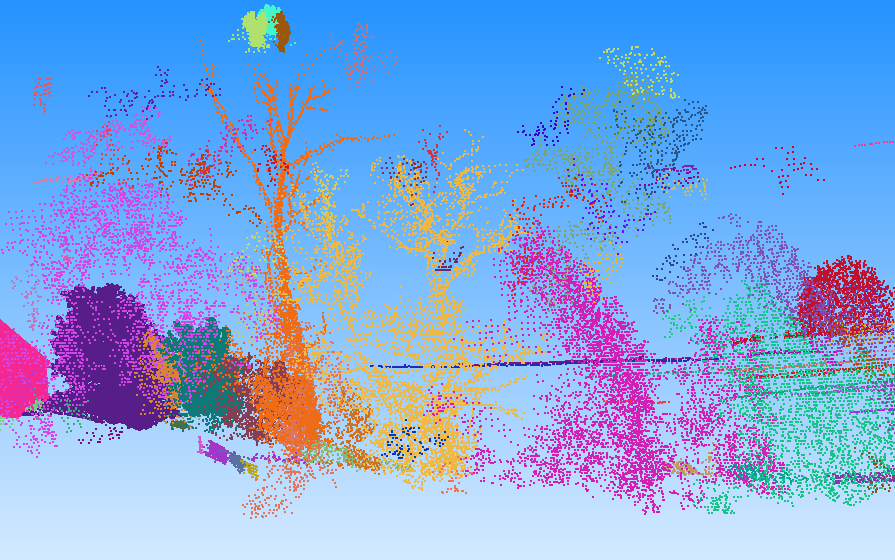
\includegraphics[width=0.45\textwidth]{3dreshaper.png}
\caption{Distance clustering \cite{Technodigit2012}}
\label{fig:dist}
\end{figure}

\begin{figure}[htb]
\centering

\includegraphics[width=0.45\textwidth]{vrmesh.png}
\caption{Automated segmentation of vegetation \cite{VirtualGrid2012}}
\label{fig:trees}
\end{figure}

\begin{table*}
\centering
  \begin{tabular}{| l | x{3cm} | x{3cm} | x{3cm} | c |}
  	\hline
	 & \multicolumn{3}{|c|}{Segmentation feature} & \\
	 \hline
	Package name & Simple & Intelligent & Auto & Open source \\    
    \hline
	Terrascan \cite{Terrasolid2012} & & & ground points, vegetation, buildings &	\tickNo \\
	\hline
	Pointools Edit \cite{Pointools2012} & lasso select\newline rectangle select, ball/cube brush select & fill select with distance threshold, fill with colour or intensity similarity, plane select & &	\tickNo \\
	\hline
	VR Mesh Studio \cite{VirtualGrid2012} & & power lines & ground, vegetation, roofs, planes &	\tickNo \\
	\hline
	Carlson PointCloud \cite{Carlson2012} & & & clear isolated and duplicate points, extract bare earth &	\tickNo \\
	\hline
	3D Reshaper \cite{Technodigit2012} & lasso select & & clustering with distance metric, clustering colours, remove isolated points &	\tickNo \\
	\hline
	Cyclone \cite{Leica2012} & lasso select & fill with smoothness similarity &  &	\tickNo \\
	\hline	
	Meshlab \cite{VisualComputingLaboratory2012} & plane select, single point select & & isolated point removal &	\tickYes \\
	\hline
  \end{tabular}
  \caption{Existing systems}
\end{table*}




Global segmentation or classification schemes can remove a lot of the effort associated with point cloud cleaning. In 3DReshaper \cite{Technodigit2012}, a point clustering approach is used to isolate distinct objects based on the distance between neighbouring points. However, because the point density of a laser scan usually decreases as points fall away from the scanner, this approach tends to produce large clusters close to the origin, and many small groups of clusters further away. Automated classification schemes take higher dimensional features into account in order to identify clusters corresponding to ground points, vegetation and buildings \cite{Terrasolid2012,VirtualGrid2012,Carlson2012}. While this may be of great for land surveyors or architects, such fully automated methods tend to lack the precision required for cultural heritage purposes.

There is certainly room to reduce the amount of productivity one has to sacrifice for precision, especially in open source tools. Meshlab \cite{VisualComputingLaboratory2012}, is currently the only known open source system that provides point cloud cleaning features. It is primarily aimed at processing triangulated meshes and therefore lacks some raw point cloud cleaning features. The recently introduced point editing features, such as point picking and plane selection, performs somewhat sluggish on larger point clouds, and are not very efficient.

%resolution of the scans are also different
% rotation table is highre
% land surveying is lower
% current workflow, select points into new layers using selection tools
% layers slow down

% no tools have been created specifically for this purpose
% cleaning can be done at various stages
% different cost benefits at different parts of the pipeline
% Meshlab, Meshedit

% system should take intensity values into account


\subsection{Related work}

% complex geopmetry cannot be discarded
% what is the model is simplified and then mapped to the complex voints
% multi resolution kind of
 Automated point cloud segmentation is not a new problem. There is however, very little available research related to the segmentation of cultural heritage data. Some success has been achieved in automatically segmenting sites into surfaces and edges through the use of Principle Component Analysis \cite{Spina2010}. What makes the segmentation of heritage data hard, is that scanned structures can exhibit very complex geometries that is hard to classify \cite{Spina2010}.

%seperate trees for sites

%Segmentation algorithms generally have two passes. The first pass sees that individual points are classified. In the second pass, segmentation is performed by grouping point features into groups that correspond to objects or parts thereof.

% What is the difference between point classification and point segmentation

%Segmentation means to divide up the image into a 
%patchwork of regions, each of which is “homogeneous”, 
%that is, the “same” in some sense
%– Intensity, texture, colour, …
%• Classification means to assign to each point in the image 
%a tissue class, where the classes are agreed in advance
%– Grey matter (GM), White matter (WM), cerebrospinal fluid (CSF), 
%air, … in the case of the brain

A variety of point feature schemes that are used extensively in robotics, could potentially be exploited in the cultural heritage domain. A number of popular point feature algorithms have been implemented and is freely available in the Point Cloud Library \cite{Rusu2011}. These include Fast Point Feature Histograms, Spin images, Global Fast Point Feature Histogram \cite{Rusu2011}.

Classification can be achieved by though either heuristic schemes \cite{Spina2010} or probabilistic models \cite{Shapovalov2010,Rusu2009}. Approaches based on machine learning have been shown to be effective.


%\subsection{Artifacts types}
\section{Research question}
La la

\section{Aims (expand)}
Why am I doing it?

Inputs, outputs
How many points
How large do point set become
we only deal with small point sets



In collaboration with geomatics

The aim of this research is to produce a system that will allow users to clean cultural heritage data in a fast and effective manner. The focus will be on finding ways to remove the most problematic artefacts as identified by the Zamani project. In descending order of importance, the focus will thus be on removing vegetation, people, and equipment. 

Existing point feature schemes will be investigated, as well as heuristic and machine learning approaches to segmentation. In order to ensure fast response times, cleaning methods will be accelerated with OpenCL.

\section{Evaluation}

Overall:

Performance metrics
	Total time taken to clean
		Given cleaning objectives
		Measure accuracy
			Perform diff against benchmark scan
		Compare old vs new
		Prior training to account for practice effects of leica point cloud
	Time performance
		
Each tool
	Interview : Expert user opinion
		Sufficient accuracy
		Confidence information
			
Remember to try clean out points in scan 1 that was already clean in scan 2.

What about pairwise registration and scanning framework?


Quantitative study (Expert users)
	Geomatics students
	Should be experienced

The system will be evaluated in a user study. The speed and accuracy of the existing system will be compared to Zamani's current system \cite{Leica2012}. Interviews will also be conducted to assess the usability of the system.

\subsection{Milestones}
\begin{tabular}{llr}
\hline
Task & Due date \\
\hline
Research Proposal & May 2012\\
Background Chapter & October 2012\\
Technical Report & November 2012\\
System Design Chapter & December 2012\\
Implementation Chapter & March 2013\\
Conference Paper & June 2013\\
First Thesis Draft & July 2013\\
Final Draft & August 2013\\
\hline
\end{tabular}




%by comparing the time taken to clean a scan with Zamani's current system \cite{Leica2012} to the new system.

% compare on a feature to fearure basis and wholesale?

% user centered design???

% user study:
% how fast clean cloud before
% for fast clean cloud after
% qualitative overview

%cleaning should be done in real time
%user testing
%focus on the problems that will have the biggest effect in terms of time savings

% Should allow them to edit accurately on a specific subspace

%\section{Methods}
%Find and classify the problems that are most difficult and time consuming

%Chris:
%    Biggest problems are:
%		Vegetation (Hard to select trees)
%		People walking through scans
%		Boxes such as equipment lying around
%
%	Problem is that useful features are scattered across many systems
%	Systems are proprietary
%	
%Systems:
%	Cyclone:
%		Select surfaces based on smoothness metric (Fuckin slow)
%		Use lasso tool
%	Pointools
%		Brush select
%	Kubit
%	Alice labs studio clouds
%	Meshlab (really hard to select things)
%	XGRT: Deals with very large clouds
%		
%		
%Desires:
%	Intelligent select
%		Eg. select table and only select surface
%	Brush type tool (Pointools):
%		Selects points based on intensity values
%	
%	Selection tools for a variety of objects
%		How to do?
%		Enumerate all types?
%		Or create some type of dynamic learning system

\bibliographystyle{plainnat}
\bibliography{proposal}	

\end{document}
